\section[Kellerautomaten (\acs*{PDA})]{Kellerautomaten \quad\normalfont\normalsize \acf{PDA}}
\newcommand{\ConfRel}{\rhd}
\newcommand{\Zinit}{Z^\mathsf{init}}
\newcommand{\K}{\mathcal{K}}
\newcommand{\el}[3]{{\color{red!70!black}#1};{\color{blue!70!black}#2};{\color{blue!70!black}#3}}

Die im letzten Kapitel vorstellten kontextfreien Sprachen können wir bisher nur mit Hilfe von kontextfreien Grammatiken darstellen.
Für die regulären Sprachen aus Kapitel~\ref{sec:reglang} haben wir dagegen mit DEAs, NEAs, $\Eps$-NEAs, regulären Ausdrücken und regulären Grammatiken verschiedene Darstellungsformen kennengelernt.
Die Automaten hatten dabei für uns einen besonderen Reiz, da diese Darstellungsform Ähnlichkeiten mit Computern hat.
In diesem Kapitel werden wir nun den Kellerautomaten, ein Automatenmodell für die kontextfreien Sprachen, kennenlernen.

Ein Kellerautomat ist im wesentlichen ein $\Eps$-NEA, der um einen Stapelspeicher mit unbeschränkter Kapazität erweitert wurde.

Bei jedem Zustandsübergang darf der Kellerautomat das oberste Element des Stapelspeichers inspizieren und durch eine (potentiell leere) Sequenz von Elementen ersetzen.
Der Automat darf dabei die Entscheidung über den Folgezustand vom inspizierten Element abhängig machen.
Zu Beginn liegt genau ein Element, das \emph{Kellerbodensymbol}, auf dem Stapelspeicher.

Der Kellerautomat unterscheidet sich noch in einem weiteren Detail vom $\Eps$-NEA:
Es gibt keine akzeptierende Zustände. 
Der Kellerautomat akzeptiert stattdessen, wenn am Ende eines Zustandsübergangs das Eingabewort komplett gelesen wurde
und der Stapelspeicher leer ist.

Analog zu endlichen Automaten können wir auch Kellerautomaten mit Hilfe eines Zustandsdiagramms beschreiben.
Ein Beispiel ist in \autoref{pdaEvenPalindrome} dargestellt.
Alle Transitionen sind mit einem Tripel beschriftet. 
Die erste Komponente des Tripels ist dabei das gelesene Zeichen der Eingabe,
die zweite Komponente ist das vom Stapelspeicher genommene Element und
die dritte Komponente ist die Sequenz, die auf den Stapelspeicher gelegt wird.

\begin{figure}[H]\centering
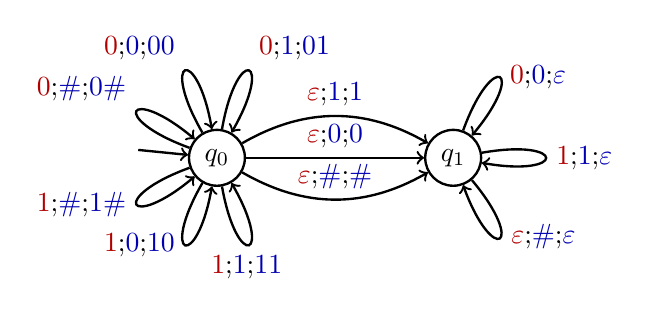
\begin{tikzpicture}[line width=0.3mm,
tape/.style={draw, node distance=0mm, minimum size=6mm, text=red!70!black, font=\bf},
tapeend/.style={node distance=0mm, minimum size=6mm, text=red!70!black, font=\bf},
stack/.style={draw=blue!50!black, node distance=0mm, minimum size=6mm, text=blue!70!black, font=\bf}
]

% \node (rect) at (0,0) [draw, rounded corners=2, fill=lightgray!20,thick,minimum width=9cm,minimum height=4cm] {};
 
 \node[circle,draw] (q1) at (-1.5,0) {$q_0$};
 \node[circle,draw] (q2) at (1.5,0) {$q_1$};
 
 
 \draw[->] (-2.5,0.1) to  (q1) ;
 
 \draw[->] (q1) edge node[auto] {\el{$\varepsilon$}{0}{0}} (q2) ;
 \draw[->, bend left] (q1) edge node[auto] {\el{$\varepsilon$}{1}{1}} (q2) ;
 \draw[->, bend right] (q1) edge node[auto] {\el{$\varepsilon$}{\#}{\#}} (q2) ;
 
 \draw[->,in=140, out=160, looseness=22, pos=0.50] (q1) edge node[auto] {\el{0}{\#}{0\#}} (q1) ;
 \draw[->,in=100, out=120, looseness=22, pos=0.50] (q1) edge node[auto] {\el{0}{0}{00}} (q1) ;
 \draw[->,in=60, out=80, looseness=22, pos=0.50] (q1) edge node[auto] {\el{0}{1}{01}} (q1) ;
 
 \draw[->,in=220, out=200, looseness=22, pos=0.50] (q1) edge node[left] {\el{1}{\#}{1\#}} (q1) ;
 \draw[->,in=260, out=240, looseness=22, pos=0.50] (q1) edge node[left] {\el{1}{0}{10}} (q1) ;
 \draw[->,in=300, out=280, looseness=22, pos=0.45] (q1) edge node[below] {\el{1}{1}{11}} (q1) ;
 

 \draw[->,in=50, out=70, looseness=22, pos=0.50] (q2) edge node[right] {\el{0}{0}{$\varepsilon$}} (q2) ;
 \draw[->,in=-10, out=10, looseness=22, pos=0.50] (q2) edge node[right] {\el{1}{1}{$\varepsilon$}} (q2) ;
 \draw[->,in=-70, out=-50, looseness=22, pos=0.45] (q2) edge node[right] {\el{$\varepsilon$}{\#}{$\varepsilon$}} (q2) ;
\end{tikzpicture}
	\caption{Zustandsdiagramm eines Kellerautomaten}
	\label{pdaEvenPalindrome}
\end{figure}

Der in \autoref{pdaEvenPalindrome} dargestellte Kellerautomat akzeptiert die Sprache $L=\{ww^R\mid w\in\{0,1\}\}$
und verwendet das Zeichen $\#$ als Kellerbodensymbol.
In Zustand $q_0$ wird für jedes Eingabezeichen das entsprechende Symbol auf den Stapelspeicher gelegt.
Zu jedem Zeitpunkt kann der Automat nichtdeterministisch (mit Hilfe einer $\Eps$-Transition) in den Zustand $q_1$ wechseln.
Diese Transition sollte genau bei der Hälfte des Eingabeworts genommen werden.
In Zustand $q_1$ vergleicht der Automat sukzessive die verbleibenden Eingabesymbole mit dem Inhalt des Stapelspeichers.
Nur bei Übereinstimmung wird der Stapelspeicher bis zum Kellerbodensymbol geleert.
Falls nur noch das Kellerbodensymbol auf dem Stapelspeicher liegt, kann der Automat dieses mit der Transition "`$\Eps;\#;\Eps$"' entfernen und die Eingabe akzeptieren.

Auf Englisch heißen Kellerautomaten \emph{pushdown automata} und wir werden die Abkürzung \ac{PDA} für Kellerautomaten verwenden. 
In diesem Kapitel befassen wir uns zunächst nur mit nichtdeterministischen Kellerautomaten und definieren diese formal wie folgt.


\begin{Def}[name={[NPDA]}]
        Ein \ac{NPDA}\footnote{Englisch: Nondeterministic Pushdown Automaton} ist ein 6-Tupel 
        $$(\Sigma,Q,\Gamma,\qinit,\Zinit,\delta).$$
        Dabei ist
        \begin{itemize}
		\item $\Sigma$, das \emph{Eingabealphabet},
                \item $Q$ eine endliche Menge von \emph{Zuständen},
                \item $\Gamma$, das \emph{Kelleralphabet},
                \item $\qinit\in Q$, der Startzustand,
                \item $\Zinit\in\Gamma$, das \emph{Kellerbodensymbol},
                \item $\delta: Q\x(\Sigma\cup\{\Eps\})\x\Gamma \-> \mathcal{P}(Q\x\Gamma^*)$ die \emph{Transitionsfunktion}. \qedhere
        \end{itemize}
\end{Def}

\begin{Bsp}\label{bsp:pda-wwr}
  Formale Beschreibung des in \autoref{pdaEvenPalindrome} abgebildeten
  Kellerautomaten. 
        \begin{align}
                \Sigma &= \{0,1\} &\qquad&\text{Eingabealphabet} \notag\\
                \Gamma &= \{0,1,\#\} &&\text{Kelleralphabet} \notag\\
                Q &= \{q_0,q_1\} &&\#\,\hat=\,\text{Kellerbodensymbol} \notag\\
                \delta(q_0,a,Z) &= \{(q_0,aZ) \}&& a\in\{0,1\},Z\in\Gamma\\
                \delta(q_0,\Eps,Z) &= \{(q_1,Z)\} \label{eq:5.2}\\
                \delta(q_1,a,a) &= \{(q_1,\Eps)\}\\
                \delta(q_1,\Eps,\#) &= \{(q_1,\Eps)\}
        \end{align}
Hat die graphische Darstellung eines Kellerautomaten sehr viele Transitionen müssen wir diese nicht alle explizit zeichnen.
Statt dessen können wir auch wie in \autoref{fig:pdaEvenPalindromeNotEplicit}
Variablen verwenden um mehrere Transitionen zusammenzufassen.
        
\begin{figure}[tp]\centering
   \begin{center}
  \begin{tikzpicture}[node distance = 3cm]
    \node[state] (0) at (0,0) {$q_0$};
    \node[node distance = 1cm, left of = 0] (start) {};
    \node[state, right of = 0] (1) {$q_1$};

    \draw[->] (start) to (0);
    \draw[->, loop above] (0) to node{$a;Z;aZ$} (0);
    \draw[->] (0) to node[auto]{$\Eps;Z;Z$} (1);
    \draw[->, loop above] (1) to node[auto]{$a;a;\Eps$} (1);
    \draw[->, loop right] (1) to node[auto]{$\Eps;\#;\Eps$} (1);
  \end{tikzpicture}
  $a\in\{0,1\}, Z\in\Gamma$
\end{center}
	\caption{Zustandsdiagramm der Kellerautomaten aus \autoref{pdaEvenPalindrome}. 
	Statt alle Transitionen explizit zu zeichnen verwenden wir die Variablen $a$ und $Z$ um eine Menge von Transitionen durch eine einzige Kante zu repräsentieren. }
	\label{fig:pdaEvenPalindromeNotEplicit}
\end{figure}
\end{Bsp}
\datenote{17.06.2026}


Im Weiteren sei $\K=(\Sigma,Q,\Gamma,\qinit,\Zinit,\delta)$ ein \ac{NPDA}.
\begin{Def}[name={[Menge der Konfigurationen eines \acs*{NPDA}]}]
        Die Menge der \emph{Konfigurationen} von $\K$ ist $\Konf(\K) = Q\x\Sigma^*\x\Gamma^*$.\\
        Die \emph{Schrittrelation} von $\K$
  \begin{displaymath}
    \mathop{\ConfRel} \subseteq \Konf(\K) \times \Konf(\K) 
  \end{displaymath}
  ist definiert durch
  \begin{align*}
    (q,aw,Z\gamma) &\ConfRel (q',w,\beta\gamma) &&\text{falls }\delta(q,a,Z)\ni(q',\beta)\\
    (q,w,Z\gamma) &\ConfRel (q',w,\beta\gamma) &&\text{falls }\delta(q,\Eps,Z)\ni(q',\beta).
  \end{align*}
  Wir schreiben $(q,w,\gamma) \ConfRel^n (q',w',\gamma')$, wenn $\K$
  in $n \in \mathbb{N}$ Schritten von Konfiguration $(q,w,\gamma)$ zur
  Konfiguration $(q',w',\gamma')$ gelangt. 

  Wir schreiben ${\ConfRel^*}$ für die reflexive, transitive Hülle
  von ${\ConfRel}$.
  % Falls $(q,w,\gamma) \ConfRel^* (q',w',\gamma')$, so existiert also
  % $n \in \mathbb{N}$, sodass $(q,w,\gamma) \ConfRel^n
  % (q',w',\gamma')$. 

  Eine  \emph{akzeptierende Konfiguration} hat die Form $(q,\Eps,\Eps)$ mit $q\in Q$.
  
  Die von $\K$ \emph{akzeptierte Sprache} ist
  \begin{displaymath}
                L(\K) = \{ w\in\Sigma^* \mid \exists q\in Q: (\qinit,w,\Zinit) \ConfRel^{\!\!*} (q,\Eps,\Eps) \}
  \end{displaymath}
\end{Def}

\begin{Bsp*}
  Die folgenden Schritte von $\K$ aus Beispiel \ref{bsp:pda-wwr} zeigen, dass $w = 0110 \in L(\K)$:
  \begin{displaymath}
  \begin{array}{r@{\ }ll}
    & (q_0, 0110, \#) \\
    \ConfRel & (q_0, 110, 0\#)  &\text{("`pushen"' des Eingabesymbols $0$)}\\
    \ConfRel & (q_0, 10, 10\#)  &\text{("`pushen"' des Eingabesymbols $1$)}\\
    \ConfRel & (q_1, 10, 10\#)  &\text{($\Eps$-Übergang von $q_0$ nach $q_1$)} \\
    \ConfRel & (q_1, 0, 0\#)  &\text{("`poppen"' des Eingabesymbols $1$)}\\
    \ConfRel & (q_1,\Eps, \#) &\text{("`poppen"' des Eingabesymbols $0$)}\\
    \ConfRel & (q_1, \Eps, \Eps) &\text{($\Eps$-Übergang zum Entfernen von $\#$)}
  \end{array}
\end{displaymath}
\end{Bsp*}

\begin{lemma}\label{lem:4.cfgToNpda}
 Zu jeder kontextfreien Sprache $L$ gibt es einen \ac{NPDA} $\mathcal{K}$, sodass $L(\mathcal{K})=L$.
\end{lemma}

Zum Führen des Beweises benötigen wir folgende Lemmas.

\begin{lemma}\label{lem:4.mehrKeller}
  Für alle $q,q' \in Q,\enspace w \in \Sigma^*,\enspace Z \in \Gamma$ und $n \in \N$ gilt:
  \begin{displaymath}
    \text{Wenn } (q,w,Z) \ConfRel^n (q', \Eps, \Eps), \text{dann } \forall v \in \Sigma^*, \gamma \in \Gamma^*: (q, wv, Z\gamma) \ConfRel^n (q', v, \gamma).
    \qedhere
  \end{displaymath}
\end{lemma}
\begin{proof}
Übungsaufgabe.
\end{proof}

\begin{lemma}\label{lem:einbettung-ableitung}
  Sei $\G= (\Sigma, N, P, S)$ eine \ac{CFG} und $\beta \vdash^*_\G
  \gamma$ eine Ableitung.

  Dann ist auch  $\alpha\beta\delta \vdash^* \alpha\gamma\delta$ eine
  Ableitung, für alle $\alpha, \delta \in (N \cup \Sigma)^*$.
\end{lemma}
\begin{proof}
  Übung oder selbst.
\end{proof}

  
\begin{proof}[von \autoref{lem:4.cfgToNpda}]
Sei $\mathcal{G} = (\Sigma,N,P,S)$ eine kontextfreie Grammatik für $L$ in \ac{CNF}.
                Definiere einen \ac{NPDA} $\mathcal{K} = (\Sigma,Q,\Gamma,\qinit,\Zinit,\delta)$ durch:
                \begin{itemize}
                        \item $Q = \{\qinit\}$ 
                        \item $\Gamma = \Sigma\overset.\cup N$
                        \item $\Zinit = S$
                        \item $\delta(\qinit,a,a) = \{(\qinit,\Eps)\} $ für $ a\in\Sigma$
                        \item $\delta(\qinit,\Eps,A) = \{(\qinit,\alpha)\}$ für $A\to\alpha\in P$
                \end{itemize}
Wir zeigen nun, dass $L(\K) = L(\mathcal{G})$.
\begin{itemize}
\item Beweisrichtung "`$\supseteq$"'
  
  Sei $w\in L(\mathcal{G})$, dann gilt $S\vdash^* w$ bzw.\ $w=Y(\T)$
  für ein $\T \in \operatorname{Abl}(S)$. Hierfür schreiben wir
  abkürzend $\T \in \operatorname{Abl}(S, w)$.
  Wir wollen zeigen, dass $(\qinit, w, S) \ConfRel^* (\qinit, \Eps,
  \Eps)$ folgt und beweisen dafür mittels Induktion über den
  zugehörigen Ableitungsbaum $\T$ die folgende
  stärkere Eigenschaft. 
  \begin{displaymath}
    \forall A \in N: \text{ wenn } \T \in \operatorname{Abl}(A, w),
    \text{dann }
    (\qinit, w, A) \ConfRel^* (\qinit, \Eps, \Eps) 
  \end{displaymath}
  Der Ableitungsbaum für $w$ hat die Form $\T = \pi (\T_1\dots\T_n)$ und wir
  führen eine Fallunterscheidung nach der Produktion $\pi$
  durch.
  \begin{itemize}
  \item $\pi = S \to \Eps$ mit $n=0$. 
    Nach Konstruktion gilt $(\qinit, \Eps) \in \delta(\qinit, \Eps,
    S)$ und somit $(\qinit, \Eps, S) \ConfRel (\qinit, \Eps, \Eps)$. 
  \item $\pi = A \to a$, $a \in \Sigma$ mit $n=0$.
    Nach Konstruktion gilt $(\qinit, a) \in \delta(\qinit, \Eps, A)$
    und $(\qinit, \Eps) \in \delta(\qinit, a, a)$. 

    Somit gilt $(\qinit, a, A) \ConfRel (\qinit, a, a) \ConfRel
    (\qinit, \Eps, \Eps)$.
  \item $\pi = A \to BC$ mit $B,C \in N$ und $n=2$.\\
   Also ist $\T = \pi(\T_1, \T_2)$,
   $\T_1 \in \operatorname{Abl}(B, u_1)$, $\T_2 \in
   \operatorname{Abl}(C, u_2)$ mit $w = u_1u_2$. 

   Nach Konstruktion gilt $(\qinit, BC) \in \delta(\qinit, \Eps, A)$. 

   Nach I.V. gilt $(\qinit, u_1, B) \ConfRel^* (\qinit, \Eps, \Eps)$
   und $(\qinit, u_2, C) \ConfRel^* (\qinit, \Eps, \Eps)$. 

        Mit \autoref{lem:4.mehrKeller} folgt schließlich:
        \begin{align*}
          (\qinit, w, A) = (\qinit, u_1u_2, A)
          &\ConfRel (\qinit, u_1u_2, BC) \\
          &\ConfRel^* (\qinit, u_2, C) \\
          &\ConfRel^* (\qinit, \Eps, \Eps).
        \end{align*}
  \end{itemize}
 \item Beweisrichtung  "`$\subseteq$"'
 
 Sei $w\in L(\K)$, dann gilt $(\qinit, w, S) \ConfRel^* (\qinit, \Eps, \Eps)$.
 Wir wollen $S \vdash^* w$ folgern und beweisen dafür mittels
 vollständiger Induktion über die Anzahl der Berechnungsschritte $n$
 die folgende Aussage: 
     \begin{displaymath}
      \forall n \in \mathbb{N}: \forall w \in \Sigma^*, \alpha \in \Gamma^*: \text{ wenn } (\qinit, w, \alpha) \ConfRel^n (\qinit, \Eps, \Eps), \text{dann } \alpha \vdash^* w
    \end{displaymath}
    
    \begin{description}
    \item[I.A.] $n = 0$.
      $w = \Eps$, $\alpha = \Eps$: Es gilt $\Eps \stackrel{*}{\vdash} \Eps$.

  \item[I.S.] $n\rightsquigarrow n+1$, $\alpha = Z\alpha'$: Betrachte
    den ersten Schritt der Berechnung
    $$(\qinit,w,Z\alpha') \ConfRel (\qinit, w', \beta\alpha') \ConfRel^n (\qinit, \Eps, \Eps),$$ 
    mit $\delta(\qinit, x, Z) \ni (\qinit, \beta)$, $x \in \Sigma \cup
    \{\varepsilon\}$. 

    Es gibt zwei Fälle für $Z$:
    \begin{itemize}
    \item $Z = a$ für $a \in \Sigma$.
%
      Es folgt $\beta = \Eps$, $w = aw'$ und $x = a$.

      Nach I.V.\ gilt $\alpha' \vdash^* w'$ und mit
      \autoref{lem:einbettung-ableitung} auch $\alpha =
      a\alpha' \vdash^* aw' = w$.  
    \item $Z = A$ mit $A \to \beta \in P$.
%
      Es folgt $w = w'$ und $x = \varepsilon$.

      Nach I.V.\ gilt $\beta\alpha' \vdash^* w'$ und somit auch
      $A\alpha \vdash \beta\alpha' \vdash^* w' = w$. 
      \qedhere
    \end{itemize}
    \end{description}
\end{itemize}
\end{proof}

\clearpage
\datenote{NEXT-UP}
Bei einem \ac{NPDA} nehmen wir in jedem Schritt ein Zeichen vom Kellerspeicher herunter,
aber dürfen beliebig viele Symbole auf den Kellerspeicher zurücklegen.
Was wäre, wenn die Höhe des Kellers pro Schritt höchstens um eins größer werden könnte?
Verlören wir dadurch nur Komfort oder könnten wir dadurch weniger Sprachen akzeptieren?

Das folgende Lemma beantwortet diese Frage.
\begin{lemma}\label{lem:4.limitStackIncrease}
        Zu jedem \ac{NPDA} gibt es einen äquivalenten \ac{NPDA}, bei dem
        für alle $q,q\in Q, Z\in\Gamma, \gamma\in\Gamma^*, x\in\Sigma\cup\{\Eps\}$
        gilt: Falls $(q',\gamma)\in\delta(q,x,Z)$, dann $|\gamma| \le 2$.
\end{lemma}
\begin{proof}
        Für jede Transition der Form $(q',\gamma)\in\delta(q,x,Z)$ mit
        $\gamma = Z_n\dots Z_1$ und $n>2$:
        \begin{itemize}
        \item Erzeuge neue Zustände $q_2\dots q_{n-1}$;
        \item Ersetze $(q',\gamma)$ durch $(q_2, Z_2Z_1)$;
        \item Definiere
          $\delta(q_i, \Eps, Z) =
          \begin{cases}
           \{ (q_{i+1}, Z_{i+1}Z_i) \} & \text{falls }x = \Eps\text{
             und }Z = Z_i \\
           \emptyset & \text{sonst;}
         \end{cases}
         $
        \item Setze $\delta(q_{n-1}, x, Z) =
          \begin{cases}
            \{ (q', Z_nZ_{n-1}) \} & \text{falls }x = \Eps\text{ und
            }Z = Z_{n-1}
            \\
            \emptyset & \text{falls }x\in\Sigma\text{ oder }Z\ne
            Z_{n-1}
            \text.
          \end{cases}
          $
        \end{itemize}
        Wiederhole, bis alle Transitionen die gewünschte Form haben.
        Die Sprache des \ac{NPDA} ändert sich durch diese Transformation nicht (ohne Beweis).\qedhere
\end{proof}


\begin{lemma}\label{lem:4.npdaToCfg}
 Zu jedem \ac{NPDA} $\mathcal{K}$ gibt es eine \ac{CFG} $\mathcal{G}$, sodass $L(\mathcal{K})=L(\mathcal{G})$.
\end{lemma}

\begin{proof}
 Ohne Einschränkung (\autoref{lem:4.limitStackIncrease}) sei $\mathcal{K} = (Q, \Sigma, \Gamma, \qinit, \Zinit, \delta)$ ein \ac{NPDA} mit $|\gamma| \le 2$ für alle $(q', \gamma) \in \delta(q, x, Z), q, q' \in Q, x \in \Sigma \cup \{\Eps\}, Z \in \Gamma$.

    Definiere $\mathcal{G} = (\Sigma, N, P, S)$ mit $N = (Q \times \Gamma \times Q) \cup \{S\}$.
    Wir wählen diese Tripel als Nichtterminalsymbole, da wir eine Grammatik konstruieren wollen, welche die folgende Eigenschaft hat:
      \begin{equation*}\label{eq:npdaToCfgProp}
        [q,Z,q']\stackrel{n}{\vdash} w \text{ gdw } (q,w,Z) \ConfRel^n (q',\Eps,\Eps) \tag{$*$}
      \end{equation*}
    In Worten: Wir können vom Nichtterminalsymbol $[q,Z,q']$ das Wort $w$ genau dann in $n$ Schritten ableiten,
    wenn der \ac{NPDA} die Konfiguration $(q,w,Z)$ in $n$ Schritten in eine akzeptierende Konfiguration mit Zustand $q'$ überführen kann.
    
    Als Menge der Regeln wählen wir $P=P_S\cup P_0\cup P_1\cup P_2$ mit:
    \begin{align*}
    P_S &= \{S \to [\qinit, \Zinit, q']\mid q'\in Q\}, \\[1mm]
    %
    P_0 &= \{ [q, Z, q'] \to x \mid (q', \Eps)\in \delta(q, x, Z), x \in \Sigma \cup \{\Eps\} \}, \\[1mm]
    %
    P_1 &= \{[q, Z, q'] \to x[q'', Z', q'] \mid (q'', Z')\in \delta(q, x, Z), q' \in Q, x \in \Sigma \cup \{\Eps\}\}, \\[1mm]
    %
    P_2 &= \{[q, Z, q'] \to x[q_1,Z_1,q_2][q_2, Z_2, q'] \mid (q_1, Z_1Z_2)\in\delta(q, x, Z), q', q_2 \in Q, x \in \Sigma \cup \{\Eps\} \}
    \end{align*}
    
    Dabei unterscheiden $P_0$, $P_1$ und $P_2$ die Fälle, dass der Stack kleiner wird ($P_0$), gleich hoch bleibt ($P_1$) oder größer wird ($P_2$).
    
    Beispiel:
    
    \ac{NPDA} für $L_\text{centered3}:=\{0^n10^n \mid n\in\N, n > 0 \}\subseteq\{0,1\}^*$:
    
    \begin{center}
    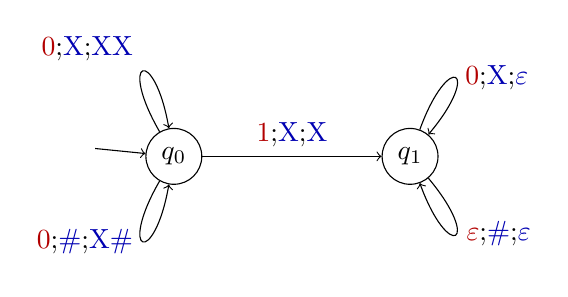
\begin{tikzpicture}
 
    \node[circle,draw] (q0) at (-1.5,0) {$q_0$};
    \node[circle,draw] (q1) at (1.5,0) {$q_1$};
    
    \draw[->] (-2.5,0.1) to  (q0) ;
    
    \draw[->] (q0) edge node[auto] {\el{1}{X}{X}} (q1) ;
    
    \draw[->,in=100, out=120, looseness=22, pos=0.50] (q0) edge node[auto] {\el{0}{X}{XX}} (q0) ;
    \draw[->,in=260, out=240, looseness=22, pos=0.50] (q0) edge node[left] {\el{0}{\#}{X\#}} (q0) ;
    
    \draw[->,in=50, out=70, looseness=22, pos=0.50] (q1) edge node[right] {\el{0}{X}{$\varepsilon$}} (q1) ;
    \draw[->,in=-70, out=-50, looseness=22, pos=0.45] (q1) edge node[right] {\el{$\varepsilon$}{\#}{$\varepsilon$}} (q1) ;
    \end{tikzpicture}
    \end{center}
    
    $010$ wird akzeptiert, weil
        $(q_0, 010, \#)\ConfRel (q_0, 10, X\#)\ConfRel (q_1, 0, X\#)\ConfRel (q_1, \Eps, \#)\ConfRel (q_1, \Eps, \Eps)$.
    
    \begin{center}
    \vspace*{-1.5\baselineskip}
    \begin{minipage}[t]{55mm}
    \begin{align*}
    P_S = \{ 
    & S \to [q_0, \#, q_0]\\
    & S \to [q_0, \#, q_1] 
    \}\\
    \\
    % \end{align*}
    % \begin{align*}
    P_0 = \{ 
    & [q_1, X, q_1] \to 0\\
    & [q_1, \#, q_1] \to \Eps
    \}\\
    \\
    % \end{align*}
    % \begin{align*}
    P_1 = \{ 
    & [q_0, X, q_0] \to 1[q_1, X, q_0]\\
    & [q_0, X, q_1] \to 1[q_1, X, q_1]
    \}
    \end{align*}
    \end{minipage}
    \begin{minipage}[t]{70mm}
    \begin{align*}
    P_2 = \{ 
    & [q_0, \#,q_0] \to 0[q_0, X, q_0] [q_0, \#, q_0]\\
    & [q_0, \#,q_0] \to 0[q_0, X, q_1] [q_1, \#, q_0]\\
    & [q_0, \#,q_1] \to 0[q_0, X, q_0] [q_0, \#, q_1]\\
    & [q_0, \#,q_1] \to 0[q_0, X, q_1] [q_1, \#, q_1]\\
    % 
    & [q_0, X,q_0] \to 0[q_0, X, q_0] [q_0, X, q_0]\\
    & [q_0, X,q_0] \to 0[q_0, X, q_1] [q_1, X, q_0]\\
    & [q_0, X,q_1] \to 0[q_0, X, q_0] [q_0, X, q_1]\\
    & [q_0, X,q_1] \to 0[q_0, X, q_1] [q_1, X, q_1]
    \}
    \end{align*}
    \end{minipage}
    \end{center}
    
    Ableitungsbaum für $010$:
    
    \begin{center}
    \vspace*{-\baselineskip}
    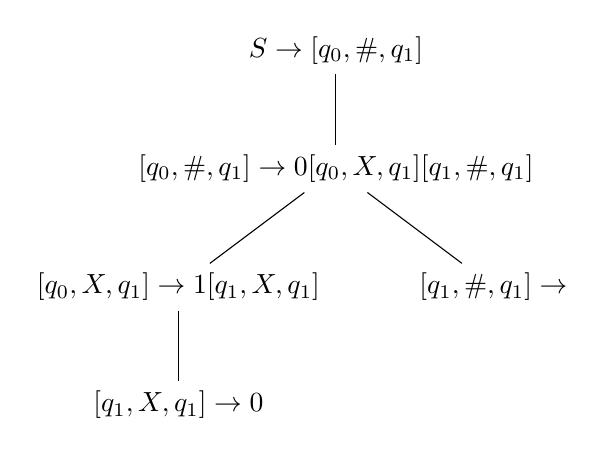
\begin{tikzpicture}
 
    \node[] (root) at (0,0) {$S \to [q_0, \#, q_1]$};
    
    \node[] (m) at (0, -1.5) {$[q_0, \#,q_1] \to 0[q_0, X, q_1] [q_1, \#, q_1]$};
    
    \node[] (ml) at (-2, -3) {$[q_0, X, q_1] \to 1[q_1, X, q_1]$};
    \node[] (mr) at (2, -3) {$[q_1, \#, q_1] \to \Eps$};
    
    \node[] (mlm) at (-2, -4.5) {$[q_1, X, q_1] \to 0$};
    
    
    
    \draw[] (root) to (m) ;
    \draw[] (m) to (ml) ;
    \draw[] (m) to (mr) ;
    \draw[] (ml) to (mlm) ;
    
    \end{tikzpicture}
    \end{center}
    
    Offensichtlich folgt aus dieser Eigenschaft $L(\mathcal{G}) = L(\mathcal{K})$, da wir vom Startsymbol $S$ genau die Nichtterminalsymbole der Form
    $[\qinit, \Zinit, q']$ ableiten können und der \ac{NPDA} genau die Wörter $w$ akzeptiert, für die  $(\qinit, w, \Zinit)$ in eine akzeptierende Konfiguration überführt werden kann.
    
    Es bleibt zu zeigen, dass die Eigenschaft \eqref{eq:npdaToCfgProp} gilt.
    Wir zeigen dafür mittels Induktion über $n$ dass für alle $n\in\N$ die folgende Eigenschaft gilt:
	\begin{equation*}
        \forall n'< n:\quad [q,Z,q']\stackrel{n'}{\vdash} w \text{ gdw } (q,w,Z) \ConfRel^{n'} (q',\Eps,\Eps) \tag{$*$}
	\end{equation*}
    
    \begin{description}
    
    	\item[I.A.] $n=1$: Folgt direkt aus den $P_0$-Regeln (und der Tatsache, dass keine der anderen Regeln ein einzelnes Symbol oder $\Eps$ ableiten kann).
    	\item[I.S.] $n\rightsquigarrow n+1$:
    	\begin{itemize}
    	 \item Beweisrichtung "`$\Rightarrow$"'
    	 
    	 Sei $[q,Z,q']\vdash\alpha\stackrel{n+1}{\vdash} w$ eine Ableitung für $w$. Für den ersten Ableitungsschritt kommen zwei Fälle in Frage:
      \begin{itemize}
      \item Fall 1: $\alpha$ hat die Form $x[q'', Z', q']$ mit $q'' \in Q$\  ($[q,Z,q']\rightarrow\alpha \in P_1$).
      
	  Dann existiert $x \in \Sigma \cup \{\Eps\}$ und $w'\in\Sigma^*$ sodass $w = xw'$ und $[q'', Z', q']\stackrel{n}{\vdash} w'$.
	  Nach I.V.\ gilt nun, dass $(q'', w', Z') \ConfRel^n (q',\Eps,\Eps)$.
	  
	  Nach Konstruktion gilt $(q'', Z')\in\delta(q, x, Z)$ und somit
	  $(q, w, Z) \ConfRel (q'', w', Z') \ConfRel^n (q',\Eps,\Eps)$.
      \item Fall 2: $\alpha$ hat die Form $x[q_1,Z_1,q_2][q_2, Z_2, q']$ ($[q,Z,q']\rightarrow\alpha \in P_2$).
      
      Es gibt also einen Ableitungsbaum $\mathcal{T} = \pi(\mathcal{T}_1,\mathcal{T}_2)$, mit $\mathcal{T}_1 \in \operatorname{Abl}([q_1, Z_1, q_2])$ und $\mathcal{T}_2 \in \operatorname{Abl}([q_2, Z_2, q'])$, sodass $w = xY(\mathcal{T}_1)Y(\mathcal{T}_2)$.
      
      Es gilt also $[q_1, Z_1, q_2]\stackrel{k_1}{\vdash} Y(\mathcal{T}_1)$ und 
      $[q_2, Z_2, q']\stackrel{k_2}{\vdash} Y(\mathcal{T}_2)$ für $k_1,k_2\in\N$, sodass $k_1+k_2=n$.
      
          Per I.V.\ folgt
          \begin{displaymath}
            (q_1, Y(\mathcal{T}_1), Z_1) \ConfRel^{k_1} (q_2, \Eps, \Eps).
          \end{displaymath}
          Mit \autoref{lem:4.mehrKeller} folgt auch
          \begin{displaymath}
            (q_1, Y(\mathcal{T}_1)Y(\mathcal{T}_2), Z_1Z_2) \ConfRel^{k_1} (q_2, Y(\mathcal{T}_2), Z_2).
          \end{displaymath}
          

      Auch hier können wir wieder I.V.\ anwenden und erhalten:
          \begin{displaymath}
            (q_2, Y(\mathcal{T}_2), Z_2) \ConfRel^{k_2} (q', \Eps, \Eps)
          \end{displaymath}
          
                    Somit gilt:
          \begin{displaymath}
            (q, \underbrace{xY(\mathcal{T}_1)Y(\mathcal{T}_2)}_{w}, Z) \ConfRel (q_1, Y(\mathcal{T}_1)Y(\mathcal{T}_2), Z_1Z_2) \ConfRel^{k_1} (q_2, Y(\mathcal{T}_2), Z_2) \ConfRel^{k_2} (q', \Eps, \Eps)
          \end{displaymath}
      \end{itemize}
      
      \item Beweisrichtung "`$\Leftarrow$"'
      Sei $(q,w,Z) \ConfRel^{n+1} (q',\Eps,\Eps)$ eine Berechnung für $w$. Da wir annehmen, 
      dass der \ac{NPDA} in einem Schritt höchstens zwei Symbole auf den Stack legen darf, kommen für den ersten Berechnungsschritt nur zwei Fälle in Frage:
      \begin{itemize}
      \item Fall 1: $(q,w,Z)\ConfRel (q'', w',Z')$ mit $w=xw'$ für $x\in\Sigma\cup\{\Eps\}$
      
      Aus $(q'', w',Z')\ConfRel^n (q',\Eps,\Eps)$ folgern wir mit I.V.\
      $[q'', Z',q']\vdash^n w'$.
      Nach Konstruktion können wir $[q,Z,q']\vdash x [q'', Z',q']$ ableiten.

      
      \item Fall 2: $(q,w,Z)\ConfRel (q_1, w',Z_1Z_2)$ mit $w=xw'$ für $x\in\Sigma\cup\{\Eps\}$

            Aus $(q_1, w',Z_1Z_2)\ConfRel^n (q',\Eps,\Eps)$ folgern wir:
      $\exists k_1,k_2\in\N, \; q_2\in Q, \; w_1,w_2\in \Sigma^*$, sodass gilt:
      \begin{enumerate}
      \item $k_1+k_2=n$
      \item $w'=w_1w_2$
      \item $(q_1, w',Z_1Z_2)\ConfRel^{k_1} (q_2, w_2,Z_2)$
      \item $(q_2, w_2,Z_2)\ConfRel^{k_2} (q',\Eps,\Eps)$
      \end{enumerate}
      Wir wählen $k_1$ als die kleinste Zahl, welche die obigen Eigenschaften erfüllt.
      Damit wissen wir, dass wir $Z_2$ noch nie vom Keller genommen haben.
      
      Aus 3.\ folgern wir $(q_1, w_1,Z_1)\ConfRel^{k_1} (q_2, \Eps,\Eps)$ und mit I.V.\
      $[q_1, Z_1, q_2] \vdash^{k_1} w_1$.
      
      Aus 4.\ folgern wir mit I.V.\ $[q_2, Z_2, q'] \vdash^{k_2} w_2$.
      
      Es gibt also einen Ableitungsbaum $\mathcal{T} = \pi(\mathcal{T}_1,\mathcal{T}_2)$, mit $\mathcal{T}_1 \in \operatorname{Abl}([q_1, Z_1, q_2])$ und $\mathcal{T}_2 \in \operatorname{Abl}([q_2, Z_2, q'])$, sodass $w = xY(\mathcal{T}_1)Y(\mathcal{T}_2)$.
      
      Somit gibt es auch eine Ableitung
      \begin{equation*}
      [q, Z, q'] \vdash x[q_1,Z_1,q_2][q_2, Z_2, q'] \vdash^{k_1+k_2} xw_1w_2. \qedhere
      \end{equation*}
      \end{itemize}
    	 
    \end{itemize}
    \end{description}

\end{proof}

\begin{Satz}
Die Menge der von Kellerautomaten akzeptierten Sprachen und die Menge der kontextfreien Sprachen sind identisch.
\end{Satz}
\begin{proof}
Folgt direkt aus \autoref{lem:4.cfgToNpda} und \autoref{lem:4.npdaToCfg}.
\end{proof}

\begin{Bemerkung}
Zu jedem \ac{NPDA} gibt es einen äquivalenten \ac{NPDA}, der nur einen Zustand hat.
(Folgt aus \autoref{lem:4.npdaToCfg} und der Konstruktion aus dem Beweis von \autoref{lem:4.cfgToNpda}.)
\end{Bemerkung}



%%% Local Variables:
%%% mode: latex
%%% TeX-master: "Info_3_Skript_SS2026"
%%% End:
